% ============================================================================
% 片G · image4 同尺并排对照（上＝源位图按源排印宽 66.3mm；下＝TikZ 重绘同宽 66.3mm）
% 编译：xelatex 片G-image4-对照-604dpi.tex → PyMuPDF 600dpi 栅格化 → PNG
% （standalone 类正文禁用 \\ / tabular，故用 minipage + \par 竖向叠放）
% 另附红/蓝叠加图（源=红、重绘=蓝、重合=黑），由 crop_g_叠加.py 生成
% ============================================================================
\documentclass[border=3mm]{standalone}
\usepackage{graphicx}
\usepackage{tikz}
\usepackage{amsmath}
\usepackage{unicode-math}
\setmathfont{texgyretermes-math.otf}
\usepackage{xeCJK}
\setCJKmainfont{SimSun}
\pagestyle{empty}
\begin{document}
\begin{minipage}{68mm}\centering
  {\small 上：源位图 image4.png（788$\times$424px，1bit 二值）按源排印宽 66.3mm 缩放}\par
  \vspace{1.2mm}
  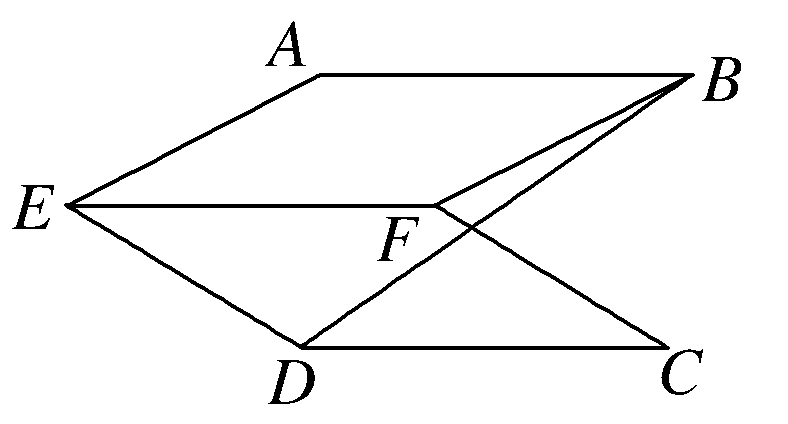
\includegraphics[width=66.3mm]{source-image4.png}\par
  \vspace{1.0mm}
  {\color[gray]{0.55}\rule{66.3mm}{0.3pt}}\par
  \vspace{1.0mm}
  {\small 下：TikZ 矢量重绘（bbox＝画布 66.3000$\times$35.6741mm，原尺寸置入 66.3mm）}\par
  \vspace{1.2mm}
  % ============================================================================
% 片G · image4 —— 二面角 A-EF-D（探八例1 题干图）TikZ 矢量重绘（逐要素复刻）
% 源位图：工作区/字替对照-0909/variantF/media/media/image4.png（788×424 px，源排印宽 66.3mm）
%
% 【折算基准】1 px = 66.3/788 = 0.0841371 mm；画布 66.3000 × 35.6741 mm
%   本片段 bbox＝源画布（含四周留白：左 1.01mm／右 3.70mm／上 1.77mm／下 1.68mm），
%   故整图等比缩放后可与现 \includegraphics 原尺寸互换：
%   VariantF body.tex 现置入宽 33.120mm ⇒ scale = 33.120/66.300 = 0.49955
%   （须连字号线宽同缩：用 \resizebox{33.120mm}{!}{…}，或 tikz 选项 scale 同步改写
%     line width 与 font 尺寸；tikz 的 scale= 不缩线宽与字号，勿单用）
%
% 【线宽】源实测笔画 4 px（灰度阈值 128，EF/AB/DC 竖切 4px、斜线横切 7~10px 换算同值）
%   ＝ 0.3365 mm ≈ 0.954 pt ⇒ 取 line width=0.34mm；线端 butt（源顶点无出锋）、拐角 miter
% 【线型】8 条实线：EF、EA、AB、FB、ED、DC、FC、DB；无虚线、无箭头、无辅助线、无标记
%   （源图连通域核算：1 个线网块 ＋ 6 个字母块，无独立短划/箭头块）
% 【标签】西文斜体数学体（源为 Times 斜体风）：源字母面高 44~46 px ⇒ 帽高 44.5 px
%   ＝ 3.7441 mm ⇒ 字号 16.03 pt（Termes 系帽高 0.662em）
%   本片段写 $A$…：在 VariantF 现行 unicode-math＋texgyretermes-math 下观感同源；
%   纯 tikz 环境编译则落 CM 斜体，几何位置不变（字体差异见核对表 md）
% 【顶点】像素（源图，y 向下）→ TikZ（mm，y 向上）：(x_px, y_px) ↦ (0.0841371·x_px, 0.0841371·(424−y_px))
% ============================================================================
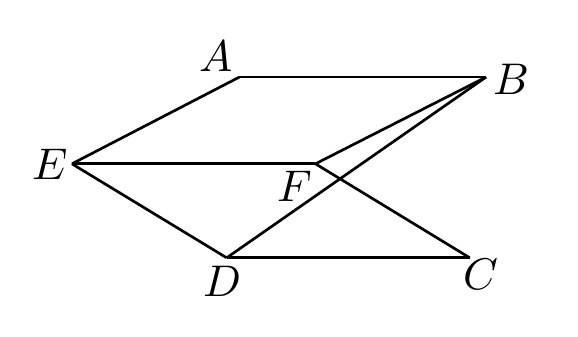
\begin{tikzpicture}[x=1mm,y=1mm,line width=0.34mm,line cap=butt,line join=miter,
                    font=\fontsize{16.03pt}{19.2pt}\selectfont]
  \path[use as bounding box] (0,0) rectangle (66.3000,35.6741);   % bbox＝源画布 788×424 px

  % ---- 顶点坐标（源 px 见行末注；由 8 条线最小二乘拟合并求交，残差 ≤0.6px） ----
  \coordinate (E) at ( 5.6204,18.3839);   % px(  66.80, 205.50)  EF∩EA
  \coordinate (A) at (26.8969,29.4059);   % px( 319.68,  74.50)  EA∩AB
  \coordinate (B) at (58.2228,29.4059);   % px( 692.00,  74.50)  AB∩FB（∩DB 得 690.87，取中）
  \coordinate (F) at (36.5491,18.3839);   % px( 434.40, 205.50)  EF∩FB（∩FC 得 435.56，取中）
  \coordinate (D) at (25.2748, 6.4470);   % px( 300.40, 347.375) ED∩DC（∩DB 得 299.17，取中）
  \coordinate (C) at (56.1463, 6.4470);   % px( 667.32, 347.375) DC∩FC

  % ---- 线（全实线，无箭头；逐条对应源图线要素） ----
  % 正方形 ABFE 四边：EF 下边、AB 上边、EA 左边、FB 右边
  \draw (E) -- (A);      % 左棱
  \draw (A) -- (B);      % 上边（源水平线 y=74.50px）
  \draw (E) -- (F);      % 公共棱 EF（源水平线 y=205.50px）
  \draw (F) -- (B);      % 右棱
  % 正方形 CDEF 四边：EF 公共棱（已画）、FC 右边、DC 下边、ED 左边
  \draw (E) -- (D);      % 左棱
  \draw (F) -- (C);      % 右棱
  \draw (D) -- (C);      % 下边（源水平线 y=347.375px）
  % 连线 BD（源图唯一交叉线：BD 与 FC 交于 px(471.4,227.4)＝mm(39.66,16.54)）
  \draw (B) -- (D);

  % ---- 标签（锚点＝源字母墨迹盒对应角，mm；inner sep=0 使锚点即字盒边） ----
  % 位置经三轮闭环标定：①按源墨迹盒角落位（残差=TeX 字盒宽/深≠墨迹盒，逐字不同）；
  % ②788px 帧互相关对齐（dx=dy=0.25px）后逐字修正；③以线网为基准逐字母亚像素微调
  % （2x 帧、0.5px@1x 步进，目标＝阈值 IoU 最大）——终态逐字母墨迹盒残差 ≤1px@1x（≤0.08mm）
  % 6 字母 + 线网的最优位移已完全一致（同为 (0,+1)px@2x），即无逐要素残余错位
  \node[anchor=south east,inner sep=0pt] at (26.1666,29.9950) {$A$};  % 源盒 px x[265,306] y[ 21, 66]
  \node[anchor=west,      inner sep=0pt] at (58.9380,29.1114) {$B$};  % 源盒 px x[702,741] y[ 57,101]
  \node[anchor=north west,inner sep=0pt] at (55.1518, 6.5206) {$C$};  % 源盒 px x[661,703] y[349,395]
  \node[anchor=north,     inner sep=0pt] at (24.6101, 5.5531) {$D$};  % 源盒 px x[268,315] y[360,404]
  \node[anchor=east,      inner sep=0pt] at ( 4.9220,18.2998) {$E$};  % 源盒 px x[ 12, 54] y[185,229]
  \node[anchor=north,     inner sep=0pt] at (33.5285,17.5847) {$F$};  % 源盒 px x[377,419] y[217,261]
\end{tikzpicture}%
% 注：末行 % 必需——\input 时尾随换行会成空格 token，被 standalone/preview 计入裁切框（实测 +3.33pt 页宽）。
\par
\end{minipage}
\end{document}
